\section{Introduction and Fundamentals}
\frame{\tableofcontents[currentsection]}
	\subsection{Introduction}
	\begin{frame}
		\frametitle{Introduction}
		\begin{itemize}
			\item Aim of this thesis:
		\begin{itemize}
			\item Verification of CNS extension for BoSSS for inviscid flows
			\item Validation for viscid flows
			\item Both using immersed boundaries
		\end{itemize}
		\item CNS extension of BoSSS (Bounded Support Spectral Solver) numerically solves the Compressible Navier-Stokes equations using a Discontinuous Galerkin method
		\item CNS has already been verified and validated for:
		\begin{itemize}
			\item Inviscid flows using immersed boundaries by \cite[Müller 2014]{muller2014}, though not for the flow around a cylinder
			\item Viscid flows using curved elements by \cite[Ayers 2015]{ayers2015}
		\end{itemize}
		\end{itemize}
	\end{frame}
	\begin{frame}
		\frametitle{Flow Properties}
		\begin{itemize}
			\item Compressible flow
			\item Ideal gas 
			\begin{itemize}
				\item Heat capacity ratio $\gamma = \dfrac{c_p}{c_v} = 1.4$
			\end{itemize}
			\item Newtonian fluid
			\begin{itemize}
				\item Stress tensor $\tau_{ij} = \mu \left[\left(\dfrac{\partial u_i}{\partial x_j} + \dfrac{\partial u_j}{\partial x_i}\right)- \dfrac{2}{3}\dfrac{\partial u_k}{\partial x_k} \delta_{ij}\right]$
			\end{itemize}
			\item Mach number $\text{Ma} = \dfrac{v_\infty}{a_\infty} = 0.2$
			\item Reynolds number $\text{Re} = \dfrac{\rho_\infty V_\infty L}{\mu_\infty} \propto \dfrac{\text{inertia forces}}{\text{viscous forces}}$
			\item Prandtl number $\text{Pr} = \dfrac{ \mu_\infty c_p}{k_\infty} \propto \dfrac{\text{viscous diffusion rate}}{\text{thermal diffusion rate}}$
		\end{itemize}
	\end{frame}
	\begin{frame}
		\frametitle{Non-dimensional 2D Compressible Navier-Stokes Equations}

%		time discretisation durch Runge-Kutta erster Ordnung -> expliziter Euler
\vspace{-0.5cm}
\begin{itemize}
	\item 2D
	\item Non-dimensional conserved flow variables: density $\rho$, momentum $\rho u$, $\rho v$, energy $\rho E$
\end{itemize}
\vspace{-0.3cm}
	\scalebox{0.9}{
		\begin{minipage}{\the\textwidth}
		\begin{align*}
			\tcbhighmath[drop fuzzy shadow,colframe=myblue]{\dfrac{\partial U}{\partial t}}+\tcbhighmath[drop fuzzy shadow,colframe=mygreen]{ \left(\dfrac{\partial F_c^x(U)}{\partial x} + \dfrac{\partial F_c^y(U)}{\partial y}\right)} - \tcbhighmath[drop fuzzy shadow,colframe=myred]{\left( \dfrac{\partial F_v^x(U, \nabla U)}{\partial x} + \dfrac{\partial F_v^y(U, \nabla U}{\partial y}\right)} = 0 			
		\end{align*}
	\end{minipage}
	}
	\begin{columns}[t]
		\begin{column}{0.6\textwidth}
			%\column[t]{7cm}
			\scalebox{0.75}{
			\begin{minipage}{\the\textwidth}
			\begin{flalign*}
			U &=\left(\begin{array}{c} \rho\\	\rho u\\ \rho v\\ \rho E\\	\end{array} \right) \quad 
			F_c^x=\left(\begin{array}{c} \rho u\\	\rho u^2 +p\\ \rho u v\\ u(\rho E +p)\\	\end{array} \right) \quad 
			F_c^y=\left(\begin{array}{c} \rho v\\	\rho u v\\ \rho v^2 +p\\ v(\rho E +p)\\	\end{array} \right) \\[8pt]
			F_v^x &= \dfrac{1}{\text{Re}}\left(\begin{array}{c} 0\\	\tau_{xx}\\ \tau_{xy}\\ \tau_{xx} u + \tau_{xy} v + \dfrac{\gamma}{\text{Pr}(\gamma - 1)}\kappa\dfrac{\partial T}{\partial x}\\	\end{array} \right) \quad
			F_v^y = \dfrac{1}{\text{Re}}\left(\begin{array}{c} 0\\	\tau_{xy}\\ \tau_{yy}\\ \tau_{xy} u + \tau_{yy} v + \dfrac{\gamma}{\text{Pr}(\gamma - 1)}\kappa\dfrac{\partial T}{\partial y}\\	\end{array} \right)
			\end{flalign*}			
		\end{minipage}
	}
	\end{column}
	\begin{column}{0.35\textwidth}
		%	\column[t]{5cm}
	\vspace{-2cm}
	\begin{itemize}
		\bluedot Temporal derivative
		\greendot Convective fluxes
		\reddot Viscous fluxes
	\end{itemize}
\end{column}
\end{columns}

	\end{frame}
	\subsection{The Discontinuous Galerkin Method}
	\begin{frame}
		\frametitle{The Discontinuous Galerkin Space Discretisation}
		\begin{columns}[t]
			\column[]{8.2cm}
			\vspace{-0.5cm}
			\begin{itemize}
				\item Discrete weak formulation of $\dfrac{\partial c}{\partial t} + \nabla \cdot \boldsymbol{f}(c) = 0 $
				\item Discretisation $\Omega_h$ of $\Omega$
				\item Multiplication of PDE by set of cell-local test functions $\Phi_{i,j}$
				\item Integration over cell $\mathcal{K}_i$ and integration by parts
				\item Modal approximation for $c(\mathbf{x} , t)\mid _{\mathcal{K}_i} \approx \sum_{k = 0}^{M}c_{i,k}(t) \Phi_{i,k}(\mathbf{x})$ with Galerkin approach (identical Ansatz and test functions)
				\item Discontinuous approach \MVRightArrow \, flux function $f = f(c^-, c^+, \mathbf{n})$
			\end{itemize}
			\vspace{-0.3cm}
			\scalebox{0.8}{
			\begin{minipage}{\the\textwidth}
			\begin{align*}
			\Rightarrow \int\limits_{\mathcal{K}_i} \dfrac{\partial c_i}{\partial t}\Phi_{i,j} \, dV +
			\sum_{e=1}^{E_i}\int\limits_{\mathcal{E}_{i,e}} f \left( c^-, c^+, \mathbf{n} \right) \Phi_{i,j} \, dA - \int\limits_{\mathcal{K}_i} \boldsymbol{f}\left(c_i\right) \cdot \nabla\Phi_{i,j} \, dV = 0
			\end{align*}
		\end{minipage}
	}
			\column[]{3.8cm}
			\begin{figure}[ht]
				%\centering
				\vspace{-1cm}
				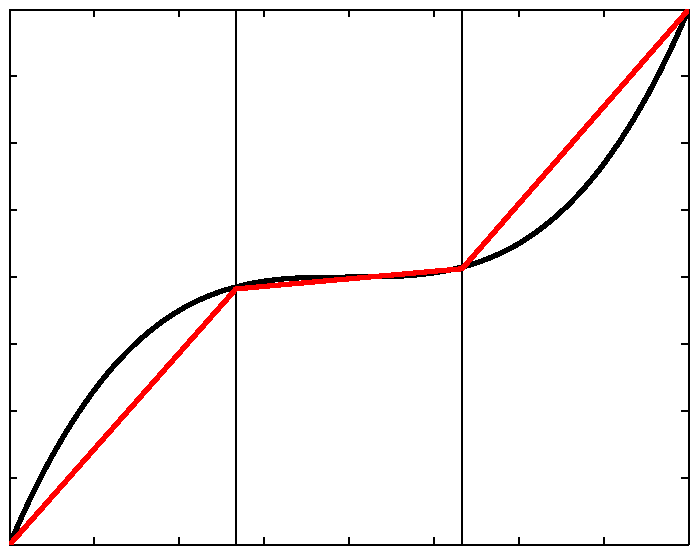
\includegraphics[height=0.31\textheight]{img/fem_cropped.pdf}
			%	\caption{First order FEM}
			\end{figure}
			\begin{figure}[htbp]
				\vspace{-0.6cm}
				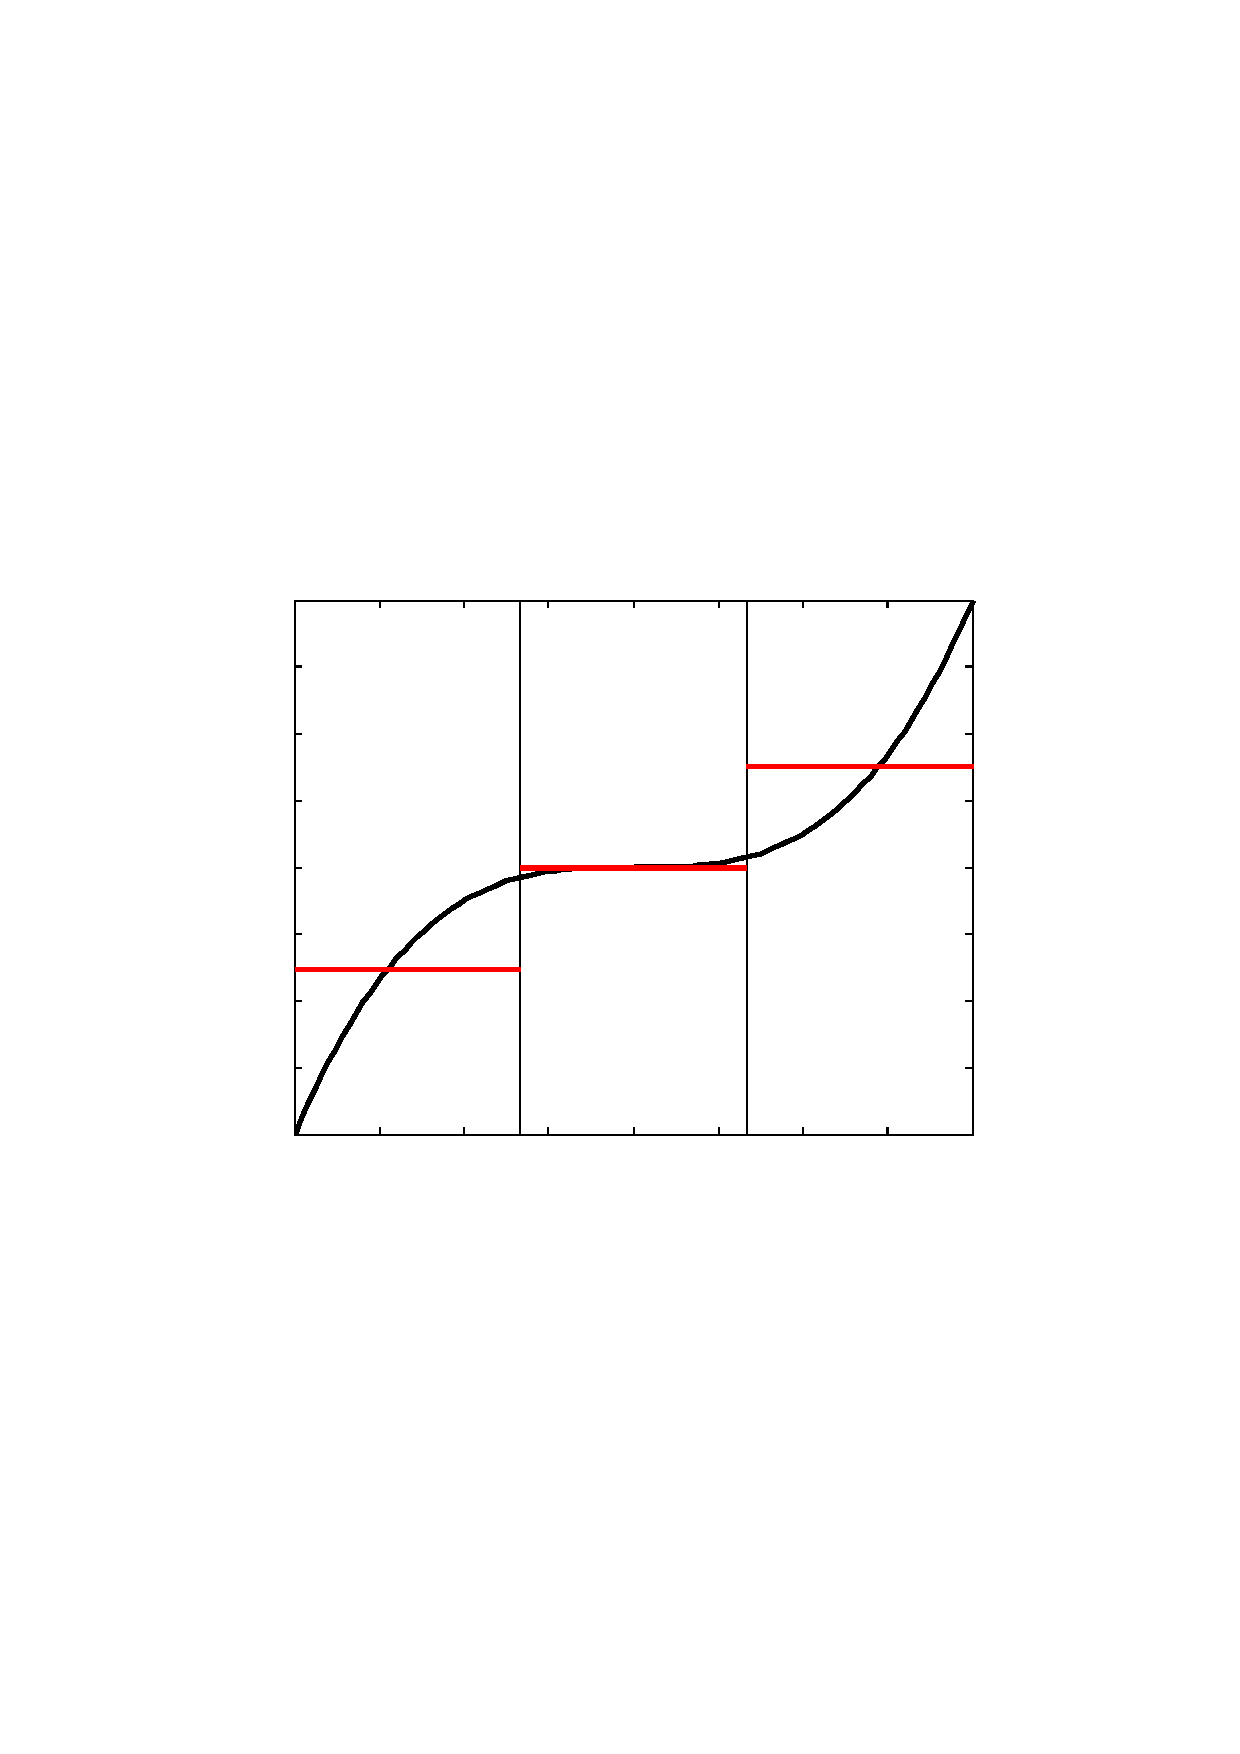
\includegraphics[height=0.31\textheight]{img/fvm.pdf}
				%\caption{Zeroth order DG (FVM) }
			\end{figure} 
			\begin{figure}[htbp]
				\vspace{-0.6cm}
				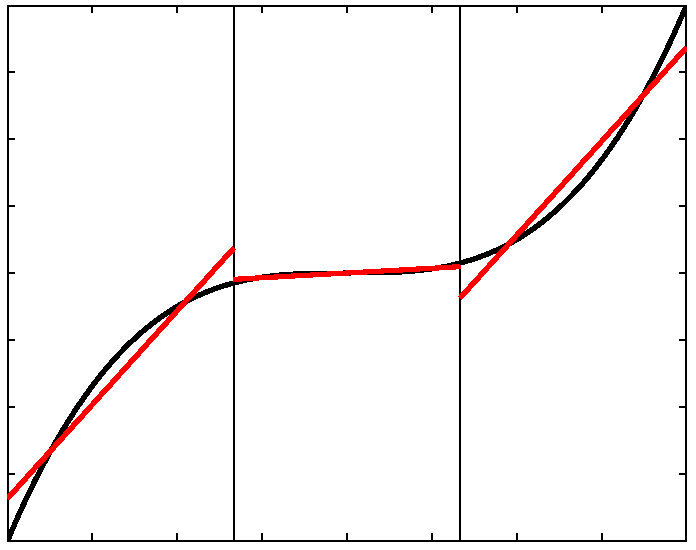
\includegraphics[height=0.31\textheight]{img/dg.pdf}
				\vspace{-0.1cm}
				\caption{Adapted from \cite{muller2014}}
			\end{figure} 
		\end{columns}
	\end{frame}
%		\begin{figure}
%			\centering
%			\subfloat[First order FEM \label{fig:a}]{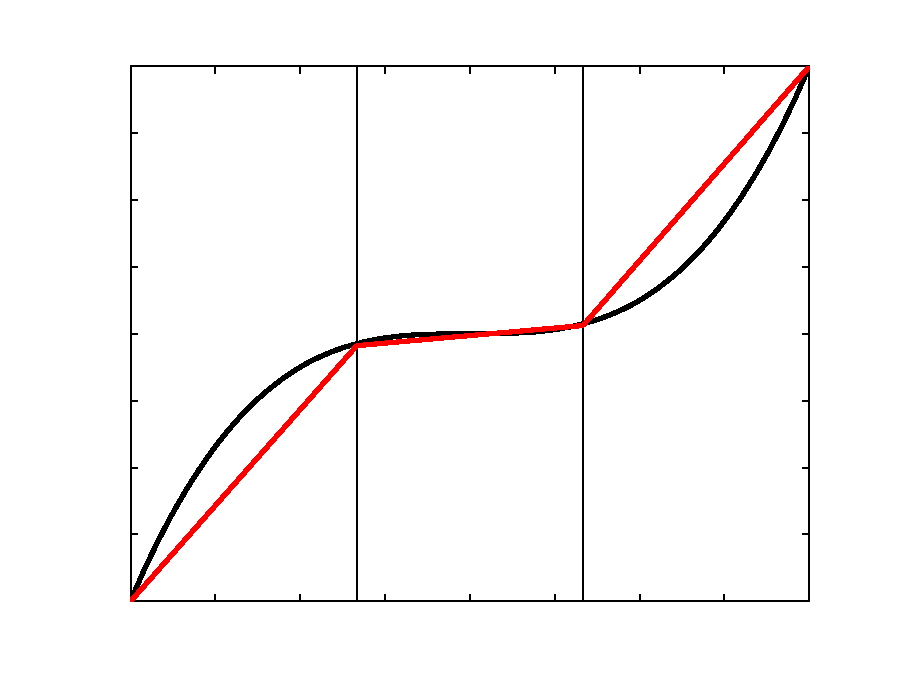
\includegraphics[width=0.28\textwidth]{img/fem.eps}}
%			\subfloat[Zeroth order DG (FVM)\label{fig:b}]{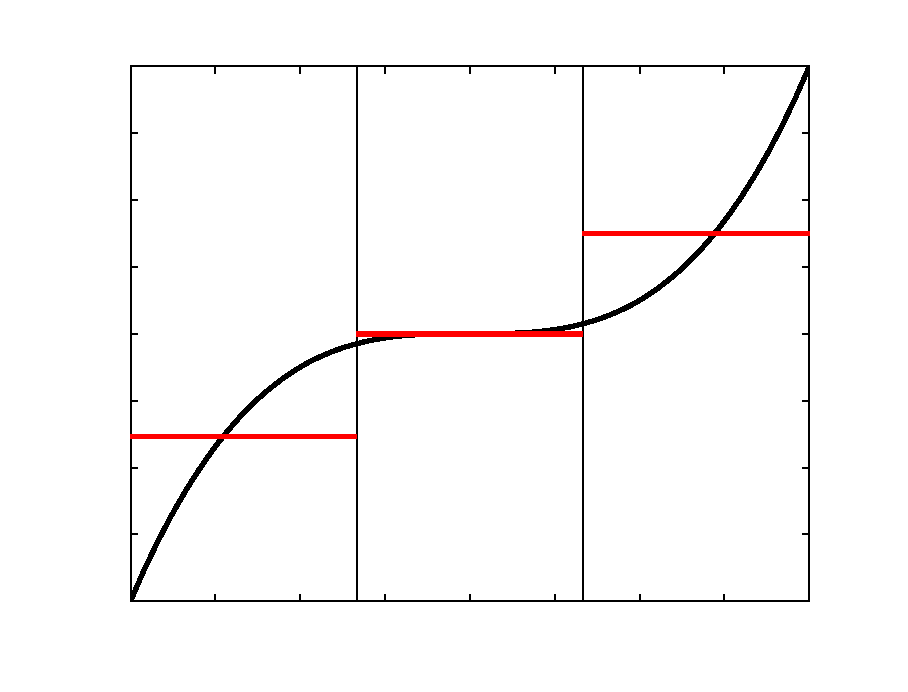
\includegraphics[width=0.28\textwidth]{img/fvm.eps}}
%			\subfloat[First order DG \label{fig:c}]{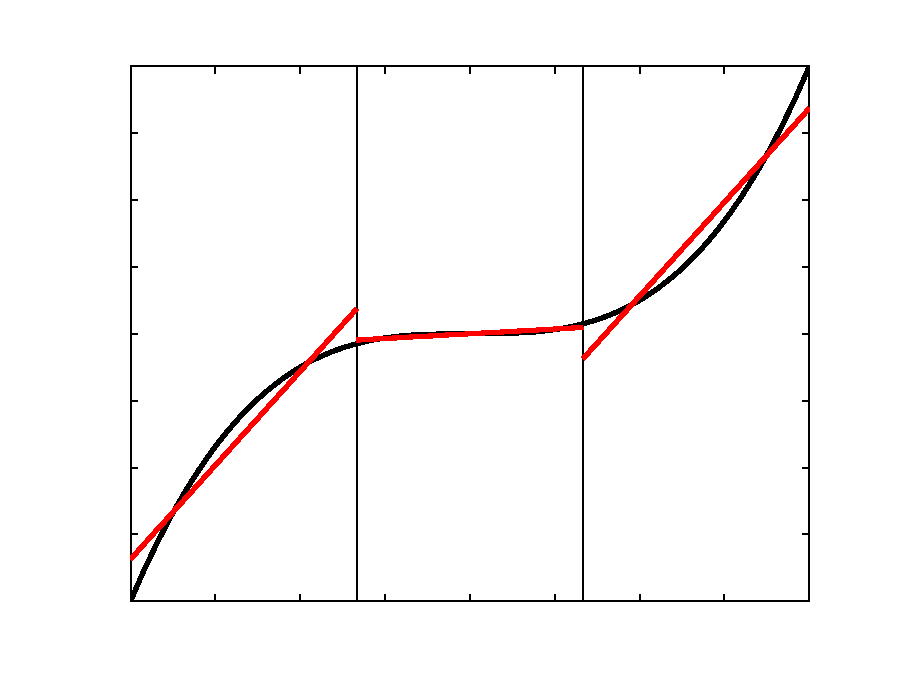
\includegraphics[width=0.28\textwidth]{img/dg.eps}}
%			\caption{Comparison of FEM, FVM and DG}
%			\label{fig:1}
%		\end{figure}
%		\begin{itemize}
%			\item Discrete weak formulation of $\dfrac{\partial c}{\partial t} + \nabla \cdot \boldsymbol{f}(c) &= 0 $
%			\item Discretisation $\Omega_h$ of $\Omega$
%			\item Multiplication of PDE by set of cell-local test functions
%			\item Integration over cell $\mathcal{K}_i$ and integration by parts
%			\item Modal approximation for $c(\mathbf{x} , t)\mid _{\mathcal{K}_i} \approx \sum_{k = 0}^{M}c_{i,k}(t) \Phi_{i,k}(\mathbf{x})$ with Galerkin approach (identical Ansatz and test functions)
%			\item Discontinuous approach \MVRightArrow \, flux function $f = f(c^-, c^+, \mathbf{n})$
%		\end{itemize}

%		DG space discretisation Vorgehen, Bildchen, fluxes

	\subsection{The Immersed Boundary Method}
	\begin{frame}
		\frametitle{The Immersed Boundary Method}
		\begin{columns}[t]
			\column[]{7cm}
			\vspace{-0.5cm}
			\begin{itemize}
				\item Division into
					\begin{itemize}
						\item the physical region:  $\mathcal{A} = \left\{\vec{x} \in \Omega_h : \varphi (\vec{x}) > 0 \right\}$,
						\item the void region:  $\mathcal{B} = \left\{ \vec{x}\in \Omega_h : \varphi (\vec{x}) < 0 \right\}$, 
						\item the immersed boundary: $\mathcal{I} = \left\{ \vec{x}\in \Omega_h : \varphi (\vec{x}) = 0 \right\}$
					\end{itemize} 
			\end{itemize}
			\column[]{5cm}
			\begin{figure}[htbp]
				\vspace{-1cm}
				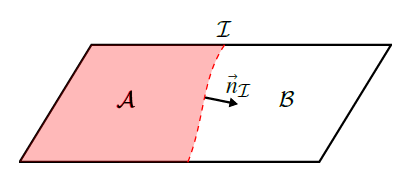
\includegraphics[width=\textwidth]{img/ibmcut.PNG}
				\caption{Cut cell with physical (red) and void region (white) \cite{paper}}\label{fig:cutcell}
			\end{figure} 
		\end{columns}
		\begin{itemize}
			\item Restrict problem domain to physical region:
		\end{itemize}
		\vspace{-0.3cm}
		\scalebox{0.9}{
			\begin{minipage}{\the\textwidth}			
				\begin{align*}
				\int\limits_{\mathcal{A}_i} \dfrac{\partial c_i}{\partial t}\Phi_{i,j} \, dV +
				\sum_{e=1}^{E_i}\int\limits_{\mathcal{E}_{i,e}^\mathcal{A}} f \left( c^-, c^+, \mathbf{n} \right) \Phi_{i,j} \, dA + \int\limits_{\mathcal{I}_{i}} f \left( c^-, c^+, \mathbf{n}_\mathcal{I} \right) \Phi_{i,j} \, dA - \int\limits_{\mathcal{A}_i} \boldsymbol{f}\left(c_i\right) \cdot \nabla\Phi_{i,j} \, dV = 0 
				\end{align*}
			\end{minipage}
			}\\
			\begin{itemize}
				\item Solution via explicit Euler time discretisation
					\begin{itemize}
						\item Time step size depends on cell with smallest volume \\
						\MVRightarrow \, Cell agglomeration
					\end{itemize}
			\end{itemize}
%		regions mit Bild, Aufteilung Integrale
%		mass matrix
%		rk time discretisation formel
%		cell agglomeration
	\end{frame}
	\begin{frame}
		\frametitle{Cell Agglomeration}

		\begin{columns}[t]
			\column[]{5cm}
			\vspace{-0.5cm}
			\begin{itemize}
				\item Agglomeration threshold  $0 \leq \alpha \leq 1$
				\item Cells $\mathcal{K}_s^\text{src}$ with $\text{frac}(\mathcal{A}_i) = \tfrac{\text{meas}(\mathcal{A}_i)}{\text{meas}(\mathcal{K}_i)} \leq \alpha$ get agglomerated to neighbouring cell $\mathcal{K}_s^\text{tar}$
				\item Neighbouring cells are weakly coupled via fluxes \newline \MVRightArrow \, basis $\vec{\Phi}_i$ can be extended from the target cell into the source cell
			\end{itemize}
			\column[]{7cm}
			\begin{figure}[htbp]
				\vspace{-1cm}
				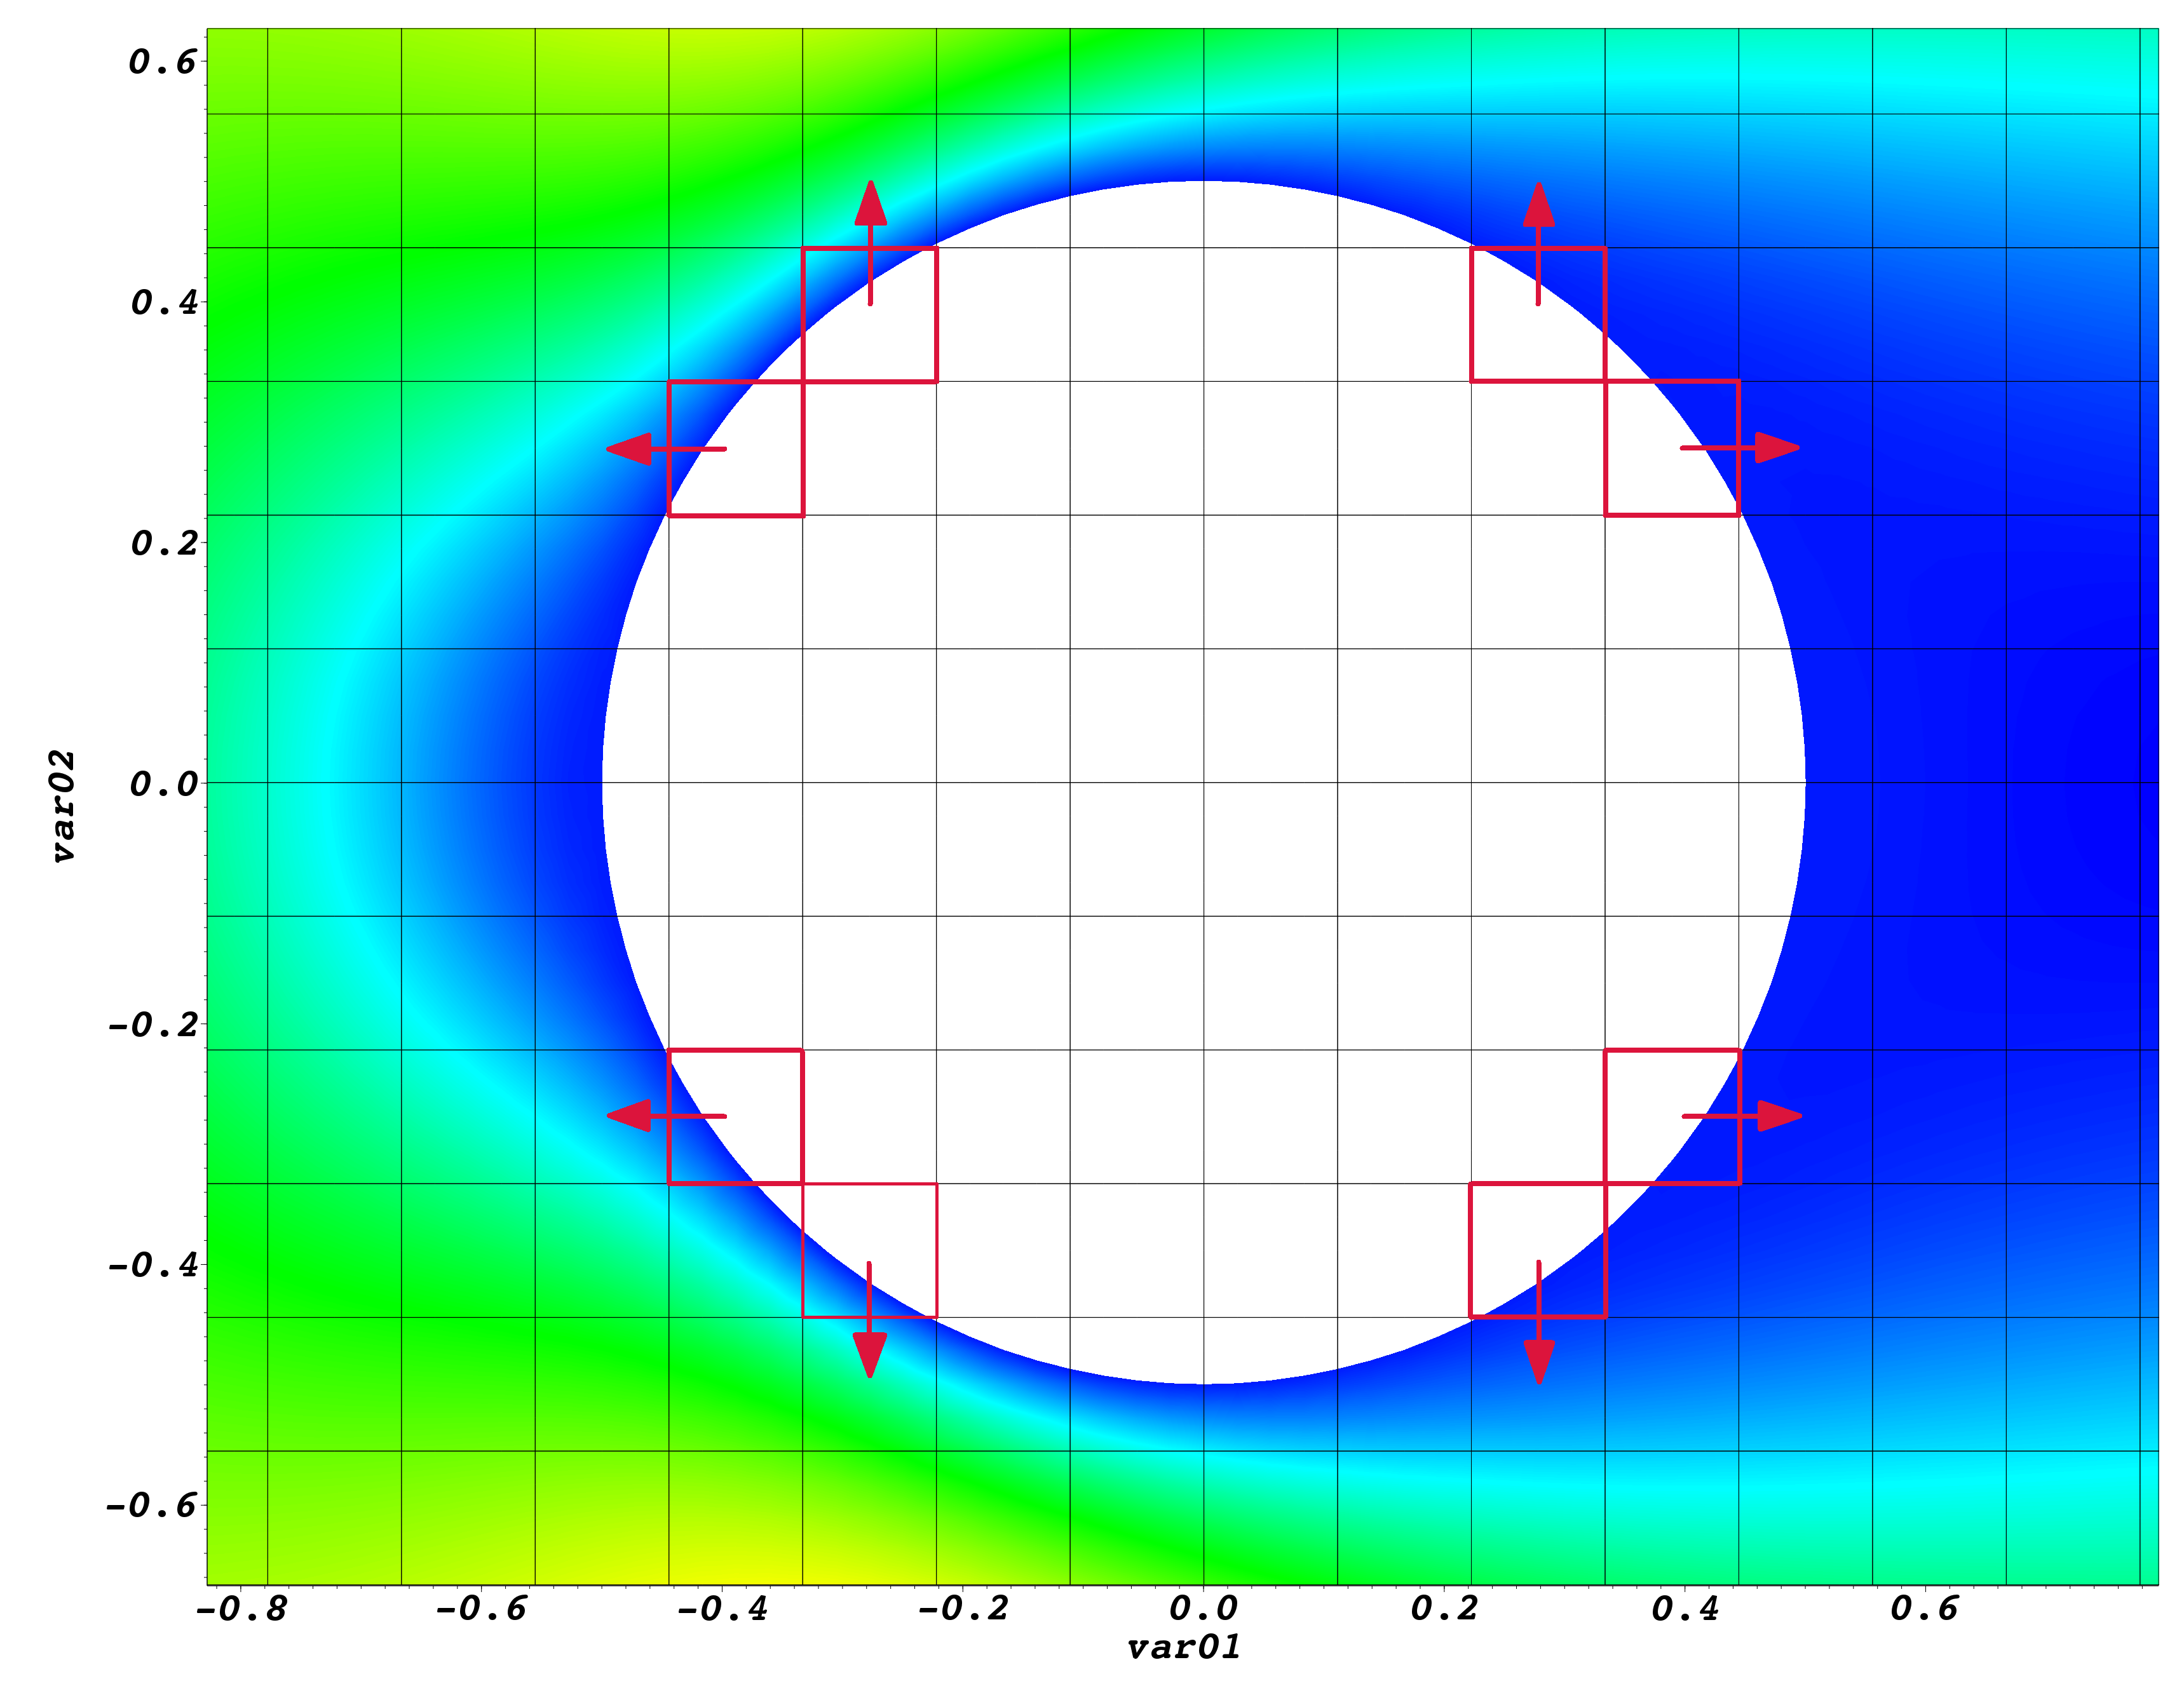
\includegraphics[width=\textwidth]{img/agglom.PNG}
				\caption{Cell agglomeration for $\alpha = 0.3$}
			\end{figure} 
		\end{columns}
%		regions mit Bild, Aufteilung Integrale
%		mass matrix
%		rk time discretisation formel
%		cell agglomeration
	\end{frame}